\chapter{विलयन और विलेयता}\label{ch:g6:solutions-and-solubility}

सोडा वॉटर की बोतल खोली जाती है: एक सिसकारी, और नन्हे बुलबुलों की एक
झड़ी न जाने कहाँ से ऊपर उठने लगती है। एक पल पहले पानी बिल्कुल स्वच्छ
दिख रहा था, फिर भी उसमें पूरे समय एक गैस घुली हुई थी। ठोस \omterm{def:g2:mixing-and-dissolving:dissolve}{घुलते} हैं, द्रव
\omterm{def:g2:mixing-and-dissolving:dissolve}{घुलते} हैं, और गैसें भी \omterm{def:g2:mixing-and-dissolving:dissolve}{घुलती} हैं --- पर कभी भी बिना सीमा के नहीं। यह
अध्याय विलयन के हिस्सों को नाम देता है और मापता है कि कोई द्रव किसी पदार्थ
की कितनी मात्रा अपने में रख सकता है।

\begin{recall}
पानी में \omterm{def:g2:mixing-and-dissolving:dissolve}{घुलने} वाला ठोस आँखों से ओझल हो जाता है और द्रव को स्वच्छ छोड़ता
है; वह स्वच्छ द्रव एक विलयन है, और जो घुला है वह अब भी उसमें मौजूद है
(\cref{ch:g2:mixing-and-dissolving})। विलयन \omterm{def:g6:pure-substances-and-mixtures:species}{रासायनिक स्पीशीज़} का एक
\omterm{def:g6:pure-substances-and-mixtures:homogeneous}{समांगी मिश्रण} है
(\cref{ch:g6:pure-substances-and-mixtures})। पानी का \omterm{def:g3:separating-mixtures:evaporate}{वाष्पन} करने से
घुला हुआ ठोस वापस मिल जाता है (\cref{ch:g3:separating-mixtures})।
\end{recall}

\begin{omfigure}
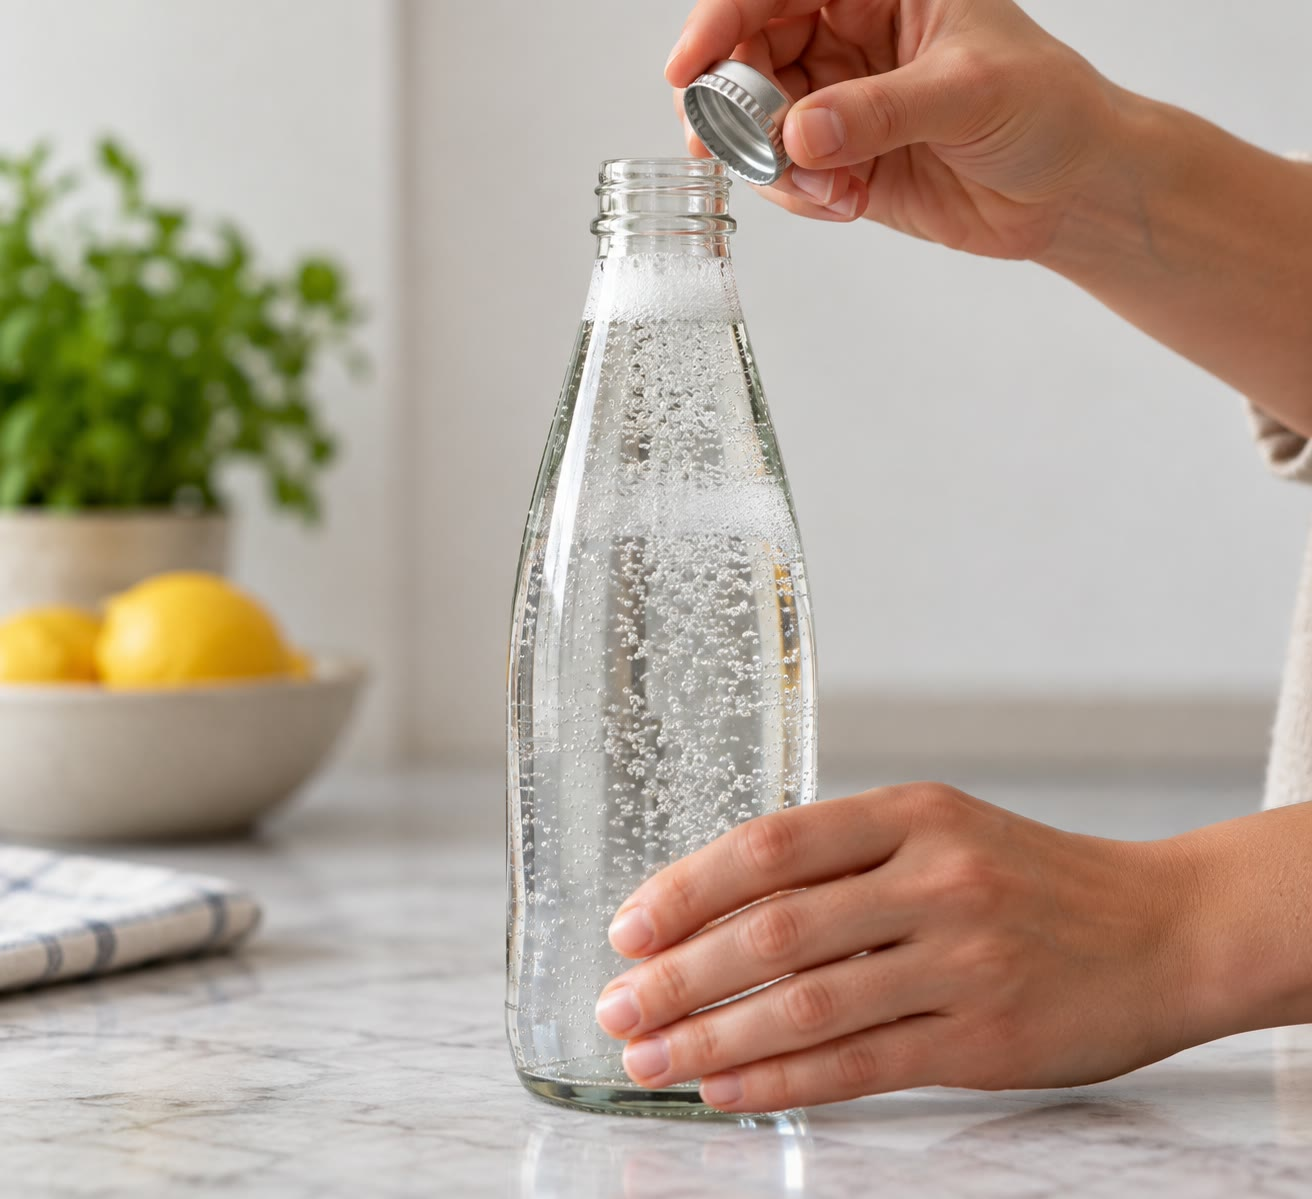
\includegraphics[width=0.5\linewidth]{images/book1/ai/g6-fizzy-water.jpg}

{\small सोडा वॉटर की बोतल खोलना: घुली हुई गैस बुलबुलों के रूप में बाहर
निकलती है।}
\end{omfigure}

\section{विलेय और विलायक}

\begin{definition}[विलेय, विलायक, जलीय विलयन]\label{def:g6:solutions-and-solubility:solute}
विलयन में जो पदार्थ \omterm{def:g2:mixing-and-dissolving:dissolve}{घुलता} है, वह
\emph{विलेय}\index{विलेय} है, और जिस द्रव में वह \omterm{def:g2:mixing-and-dissolving:dissolve}{घुलता} है, वह
\emph{विलायक}\index{विलायक} है। जब विलायक पानी हो, तो विलयन
\emph{जलीय विलयन}\index{जलीय विलयन} कहलाता है।
\end{definition}

\begin{example}[पानी के अलावा विलायक]\label{ex:g6:solutions-and-solubility:solvents}
पानी सबसे आम \omterm{def:g6:solutions-and-solubility:solute}{विलायक} है, पर अकेला नहीं। नेल पॉलिश पानी में नहीं \omterm{def:g2:mixing-and-dissolving:dissolve}{घुलती};
वह प्रोपेनोन (ऐसीटोन) में \omterm{def:g2:mixing-and-dissolving:dissolve}{घुलती} है, जो नेल पॉलिश रिमूवर का \omterm{def:g6:solutions-and-solubility:solute}{विलायक} है।
ग्रीस और तैल रंग खनिज तारपीन में \omterm{def:g2:mixing-and-dissolving:dissolve}{घुलते} हैं।
बहुत-सी दवाइयाँ एथेनॉल में घोली जाती हैं। एक विलयन में कई \omterm{def:g6:solutions-and-solubility:solute}{विलेय} हो सकते
हैं: समुद्र के पानी में घुला हुआ नमक और बहुत-से दूसरे पदार्थ होते हैं।
\end{example}

\begin{safety}{\ghs{GHS02}\ghs{GHS07}}
% ledger: ghs:acetone
प्रोपेनोन (ऐसीटोन): अत्यधिक ज्वलनशील द्रव और वाष्प (GHS02); यह आँखों में
जलन करता है और इसकी वाष्प से उनींदापन या चक्कर आ सकता है (GHS07)।
इसे हवादार कमरे में, किसी भी लौ से दूर, इस्तेमाल किया जाता है।
\end{safety}

\begin{proposition}[द्रव्यमान जुड़ते हैं]\label{prop:g6:solutions-and-solubility:mass}
विलयन का द्रव्यमान \omterm{def:g6:solutions-and-solubility:solute}{विलायक} के द्रव्यमान और घुले हुए \omterm{def:g6:solutions-and-solubility:solute}{विलेय} के द्रव्यमान का
योग होता है: ठोस के \omterm{def:g2:mixing-and-dissolving:dissolve}{घुलने} पर कुछ भी नहीं खोता, भले ही वह अब
दिखाई न दे।
\end{proposition}

\begin{omfigure}
\begin{tikzpicture}[font=\small, scale=1.15]
  \pic[transform shape] at (0,0) {balance};
  \pic[transform shape] at (0,0.8) {beaker={0.5}{omWater!80}};
  \node[anchor=north, align=center] at (0,-0.1) {\qty{100}{g} पानी};
  \node at (1.85,1.3) {$+$};
  \pic[transform shape] at (3.5,0) {balance};
  \fill[white, draw=black!45] (3.0,0.8) rectangle (4.0,0.9);
  \fill[white, draw=black!45] (3.15,0.9) -- (3.85,0.9) -- (3.5,1.2) -- cycle;
  \node[anchor=north, align=center] at (3.5,-0.1) {\qty{10}{g} चीनी};
  \draw[->, thick, omProp] (4.9,1.2) -- (6.0,1.2) node[midway, above, text=black]
    {चलाओ};
  \pic[transform shape] at (7.4,0) {balance};
  \pic[transform shape] at (7.4,0.8) {beaker={0.52}{omWater!80}};
  \node[anchor=north, align=center] at (7.4,-0.1) {\qty{110}{g} चीनी का पानी};
\end{tikzpicture}

{\small \qty{100}{g} पानी में \qty{10}{g} चीनी घोलने पर
\qty{110}{g} विलयन मिलता है (बीकर का द्रव्यमान नहीं गिना गया)।}
\end{omfigure}

\section{संतृप्ति और विलेयता}

\begin{definition}[संतृप्त विलयन]\label{def:g6:solutions-and-solubility:saturated}
कोई विलयन \emph{संतृप्त विलयन}\index{संतृप्त विलयन} होता है जब
वह अपने \omterm{def:g6:solutions-and-solubility:solute}{विलेय} की और मात्रा नहीं घोल सकता: डाला गया कोई भी \omterm{def:g6:solutions-and-solubility:solute}{विलेय}, हम कितनी
भी देर चलाएँ, बिना घुले तली में पड़ा रहता है।
\end{definition}

\begin{definition}[विलेयता]\label{def:g6:solutions-and-solubility:solubility}
किसी \omterm{def:g6:solutions-and-solubility:solute}{विलायक} में किसी \omterm{def:g6:solutions-and-solubility:solute}{विलेय} की \emph{विलेयता}\index{विलेयता} \omterm{def:g6:solutions-and-solubility:solute}{विलेय} का
वह अधिकतम द्रव्यमान है जिसे \omterm{def:g6:solutions-and-solubility:solute}{विलायक} की दी गई मात्रा, एक दिए गए ताप पर,
घोल सकती है। पानी में किसी ठोस के लिए इसे अक्सर ग्राम प्रति लीटर (या प्रति
किलोग्राम) पानी में दिया जाता है।
\end{definition}

\begin{proposition}[पानी में कुछ विलेयताएँ]\label{prop:g6:solutions-and-solubility:values}
% ledger: sol:NaCl, sol:sucrose, sol:CO2, sol:O2 (O2: 31 mL/L, 31/24.0 x 32 = 0.041 g/L at 20 C)
पानी में मापी गई \omterm{def:g6:solutions-and-solubility:solubility}{विलेयताएँ} एक-दूसरे से बहुत अलग हैं:
\begin{center}
\small
\begin{tabular}{lll}
\hline
\omterm{def:g6:solutions-and-solubility:solute}{विलेय} & पानी में \omterm{def:g6:solutions-and-solubility:solubility}{विलेयता} & परिस्थितियाँ \\
\hline
चीनी (सुक्रोस) & प्रति लीटर पानी लगभग \qty{2000}{g} & कमरे का ताप \\
नमक (सोडियम क्लोराइड) & प्रति किलोग्राम पानी \qty{360}{g} & \qty{25}{\celsius} \\
कार्बन डाइऑक्साइड & प्रति लीटर लगभग \qty{1.5}{g} & \qty{25}{\celsius}, गैस के नीचे \\
ऑक्सीजन & प्रति लीटर लगभग \qty{0.04}{g} & \qty{20}{\celsius}, गैस के नीचे \\
रेत, खड़िया & लगभग शून्य & --- \\
\hline
\end{tabular}
\end{center}
एक लीटर पानी अपने द्रव्यमान से भी ज़्यादा चीनी घोल सकता है, पर आधा ग्राम
ऑक्सीजन भी नहीं।
\end{proposition}

\begin{method}[क्या पूरा घुल जाएगा?]\label{met:g6:solutions-and-solubility:will-it}
यह जानने के लिए कि \omterm{def:g6:solutions-and-solubility:solute}{विलेय} का द्रव्यमान $m$ पानी के किसी आयतन में पूरा घुलेगा
या नहीं:
\begin{enumerate}
  \item \omterm{def:g6:solutions-and-solubility:solute}{विलेय} की \omterm{def:g6:solutions-and-solubility:solubility}{विलेयता} पता करो (ग्राम प्रति लीटर पानी में);
  \item निकालो कि पानी का यह आयतन अधिकतम कितना द्रव्यमान घोल सकता है;
  \item उसकी तुलना $m$ से करो: अगर $m$ छोटा है, तो सब कुछ घुल जाता है; अगर $m$
        बड़ा है, तो विलयन संतृप्त है और बाकी तली में
        रह जाता है।
\end{enumerate}
\end{method}

\begin{example}[गिलास में नमक]\label{ex:g6:solutions-and-solubility:glass}
% ledger: sol:NaCl
क्या \qty{50}{g} नमक \qty{200}{mL} पानी (लगभग \qty{200}{g}) में घुल
सकता है? एक किलोग्राम पानी अधिकतम \qty{360}{g} नमक घोलता है,
इसलिए \qty{200}{g} पानी अधिकतम $360 \times
\frac{200}{1000} = \qty{72}{g}$ घोलता है। चूँकि $50 < 72$, सारा नमक
घुल जाता है।
\end{example}

\begin{omfigure}
\begin{tikzpicture}[font=\small, scale=1.15]
  \pic[transform shape] at (0,0) {beaker={0.6}{omWater!80}};
  \node[anchor=north, align=center] at (0,-0.15) {थोड़ा नमक:\\ सब घुला};
  \pic[transform shape] at (3.2,0) {beaker={0.6}{omWater!80}};
  \node[anchor=north, align=center] at (3.2,-0.15) {और नमक:\\ ठीक संतृप्त};
  \pic[transform shape] at (6.4,0) {beaker={0.6}{omWater!80}};
  \fill[black!12, draw=black!50] (5.7,0) -- (7.1,0) -- (6.9,0.2) -- (5.9,0.2) -- cycle;
  \foreach \x in {5.85,6.05,6.25,6.45,6.65,6.85} \fill[black!45] (\x,0.09) circle (0.03);
  \node[anchor=north, align=center] at (6.4,-0.15) {बहुत ज़्यादा नमक:\\ बाकी बिना घुले रहता है};
\end{tikzpicture}

{\small उसी पानी में नमक बढ़ाते जाना। विलयन संतृप्त हो जाने पर
अतिरिक्त नमक तली में रह जाता है।}
\end{omfigure}

\begin{inthelab}[नमकीन पानी को संतृप्त करना]
शिक्षक \qty{100}{mL} पानी में एक-एक चम्मच नमक डालते हैं, और हर बार
अच्छी तरह चलाते हैं। पहले कुछ चम्मच ग़ायब हो जाते हैं; फिर एक चम्मच पूरा
नहीं \omterm{def:g2:mixing-and-dissolving:dissolve}{घुलता} और सफ़ेद दाने तली में रह जाते हैं: विलयन संतृप्त है। इस्तेमाल
किए गए नमक को तौलने पर पता चलता है कि लगभग \qty{36}{g} घुल चुका है।
\end{inthelab}

\section{मिश्रणीय और अमिश्रणीय द्रव}

\begin{definition}[मिश्रणीय और अमिश्रणीय द्रव]\label{def:g6:solutions-and-solubility:miscible}
दो द्रव \emph{मिश्रणीय}\index{मिश्रणीय} होते हैं जब मिलाने पर
वे एक अकेला समांगी द्रव बना दें। वे
\emph{अमिश्रणीय}\index{अमिश्रणीय} होते हैं जब वे दो परतों में अलग हो जाएँ,
हल्का द्रव ऊपर।
\end{definition}

\begin{example}[पानी के साथ एथेनॉल, पानी के साथ तेल]\label{ex:g6:solutions-and-solubility:liquids}
पानी और एथेनॉल \omterm{def:g6:solutions-and-solubility:miscible}{मिश्रणीय} हैं: साथ में हिलाने पर वे एक स्वच्छ द्रव बना देते
हैं। पानी और तेल \omterm{def:g6:solutions-and-solubility:miscible}{अमिश्रणीय} हैं: उन्हें कितना भी ज़ोर से हिलाया जाए, तेल फिर
ऊपर आकर एक अलग परत में पानी पर तैरने लगता है। सलाद ड्रेसिंग के मर्तबान में
तेल सिरके के ऊपर तैरता है, और सिरका ज़्यादातर
पानी ही है।
\end{example}

\begin{omfigure}
\begin{tikzpicture}[font=\small, scale=1.3]
  \pic[transform shape] at (0,0) {testtube={0.6}{omWater!80}};
  \node[anchor=north, align=center] at (0,-0.15) {पानी + एथेनॉल:\\ एक परत};
  \pic[transform shape] at (3,0) {testtube={0.65}{yellow!55!orange!60}};
  \begin{scope}
    \clip (2.75,3) -- (2.75,0.25) arc[start angle=180, end angle=360, radius=0.25]
      -- (3.25,3) -- cycle;
    \fill[omWater!80] (2.7,0) rectangle (3.3,1.1);
  \end{scope}
  \draw[omGlass, line width=0.7pt] (2.75,3) -- (2.75,0.25) arc[start angle=180,
    end angle=360, radius=0.25] -- (3.25,3);
  \draw[<-, omProp, thick] (3.3,1.55) -- (4.1,1.75) node[right, text=black] {तेल};
  \draw[<-, omProp, thick] (3.3,0.6) -- (4.1,0.6) node[right, text=black] {पानी};
  \node[anchor=north, align=center] at (3,-0.15) {पानी + तेल:\\ दो परतें};
\end{tikzpicture}

{\small \omterm{def:g6:solutions-and-solubility:miscible}{मिश्रणीय} द्रव एक परत देते हैं; \omterm{def:g6:solutions-and-solubility:miscible}{अमिश्रणीय} द्रव दो।}
\end{omfigure}

\begin{omfigure}
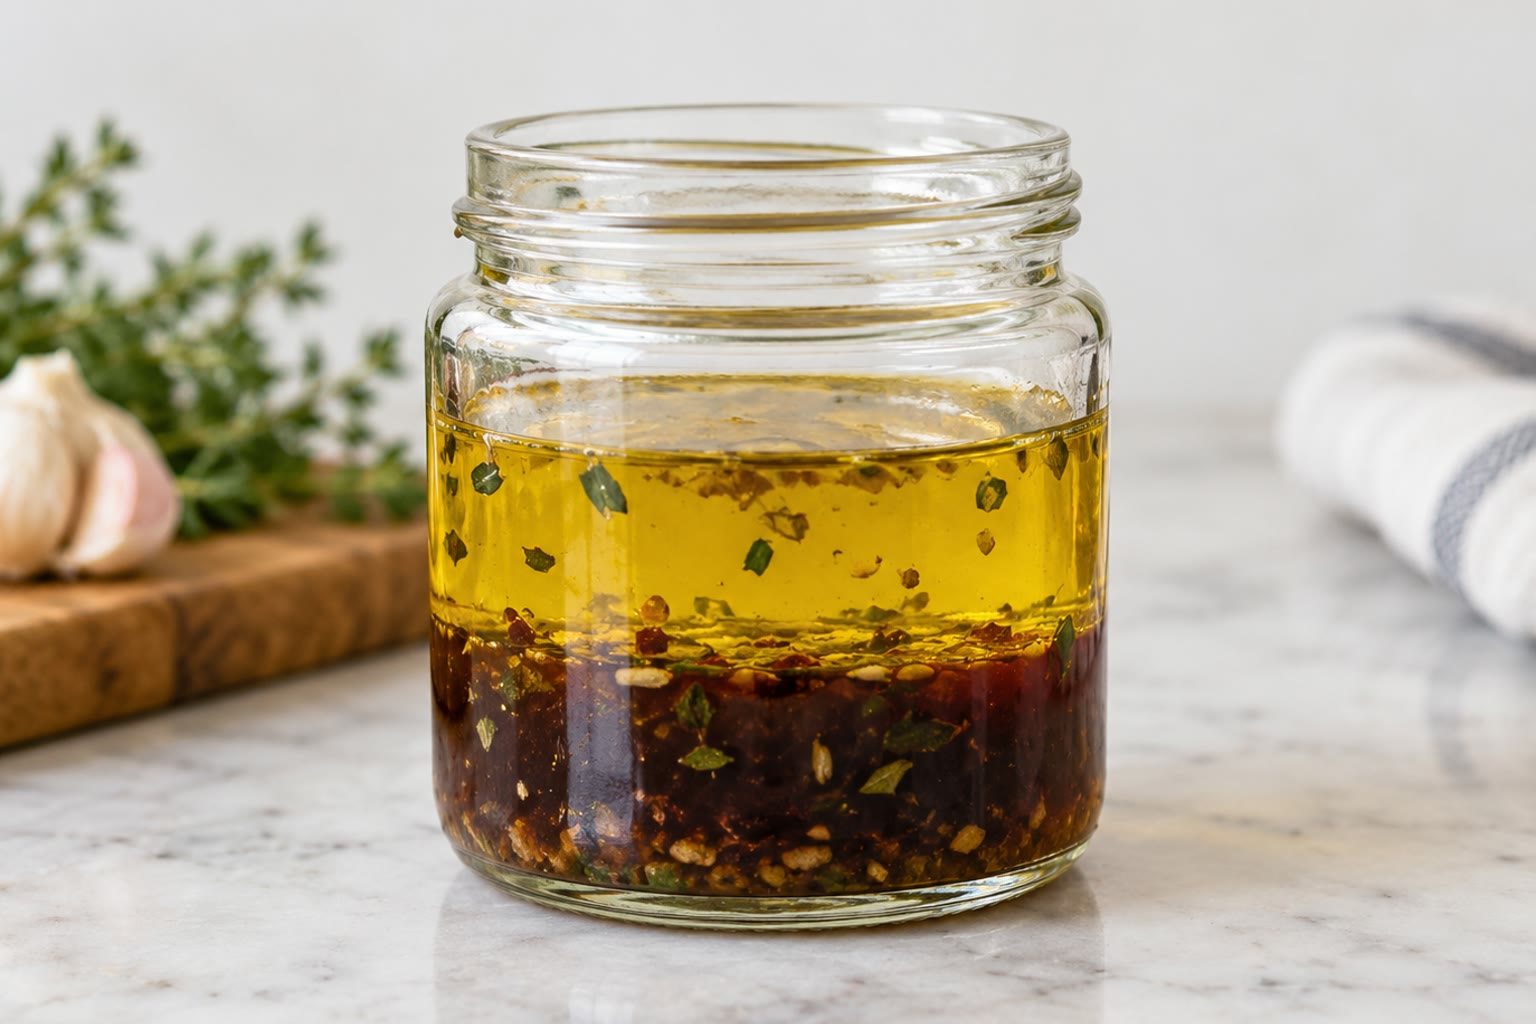
\includegraphics[width=0.45\linewidth]{images/book1/ai/g6-vinaigrette.jpg}

{\small सलाद ड्रेसिंग: तेल और सिरका \omterm{def:g6:solutions-and-solubility:miscible}{अमिश्रणीय} हैं।}
\end{omfigure}

\section{गैसें भी घुलती हैं}

\begin{proposition}[घुली हुई गैसें]\label{prop:g6:solutions-and-solubility:gases}
गैसें पानी में थोड़ी-सी \omterm{def:g2:mixing-and-dissolving:dissolve}{घुलती} हैं। सोडा वाले पेय बंद बोतल में दाब के साथ
कार्बन डाइऑक्साइड घोलकर बनाए जाते हैं; बोतल खोलने पर गैस का कुछ भाग
बुलबुलों के रूप में वापस बाहर आता है। \omterm{def:g4:air-a-mixture-of-gases:air}{वायु} के संपर्क वाले पानी में कुछ
घुली हुई ऑक्सीजन होती है, जिसे मछलियाँ अपने गलफड़ों से लेती हैं। कोई गैस
ठंडे पानी की तुलना में गरम पानी में कम \omterm{def:g2:mixing-and-dissolving:dissolve}{घुलती} है: गरम सोडा पेय जल्दी
फीका पड़ जाता है।
\end{proposition}

\begin{example}[महासागर और कार्बन डाइऑक्साइड]\label{ex:g6:solutions-and-solubility:oceans}
पृथ्वी की सतह के दो-तिहाई भाग पर महासागर \omterm{def:g4:air-a-mixture-of-gases:air}{वायु} के संपर्क में हैं। \omterm{def:g4:air-a-mixture-of-gases:air}{वायु} की
कार्बन डाइऑक्साइड उनमें \omterm{def:g2:mixing-and-dissolving:dissolve}{घुलती} है, इसलिए मनुष्य जितनी कार्बन डाइऑक्साइड \omterm{def:g4:air-a-mixture-of-gases:air}{वायु}
में छोड़ते हैं, उसका एक भाग महासागर सोख लेते हैं।
\end{example}

\begin{omfigure}
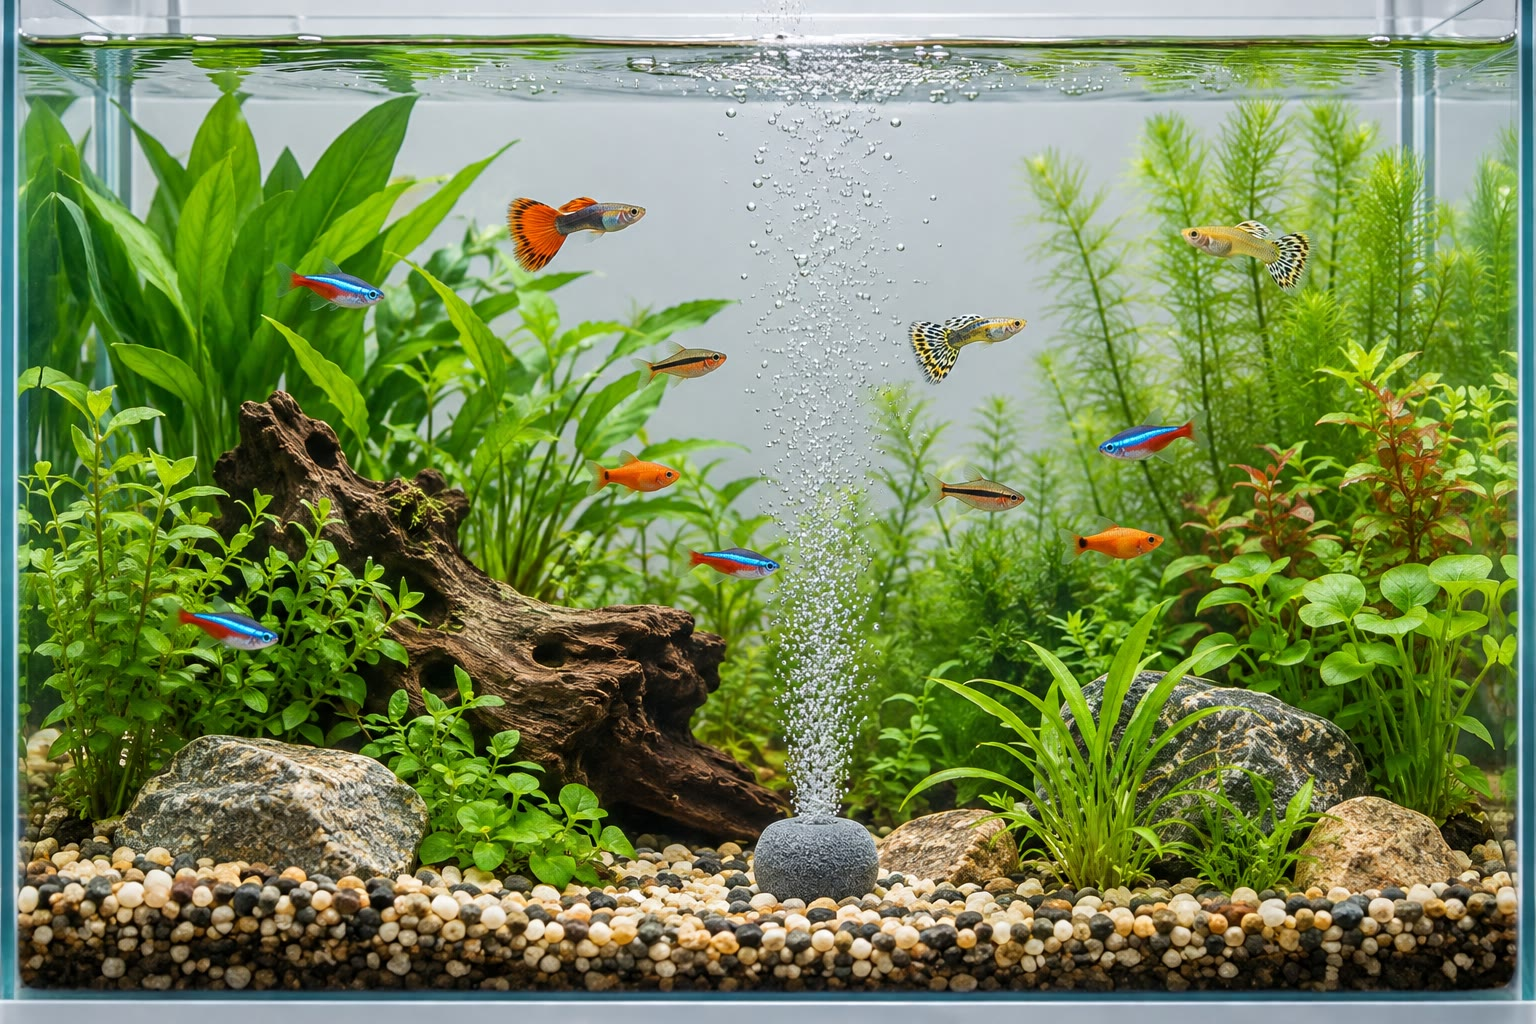
\includegraphics[width=0.5\linewidth]{images/book1/ai/g6-fish-tank.jpg}

{\small मछलीघर: \omterm{def:g4:air-a-mixture-of-gases:air}{हवा} के बुलबुले मछलियों के लिए पानी में घुली हुई
ऑक्सीजन बनाए रखते हैं।}
\end{omfigure}

\section{अभ्यास}

\begin{exercise}[$\star$]\label{exo:g6:solutions-and-solubility:1}
चीनी के पानी में \omterm{def:g6:solutions-and-solubility:solute}{विलेय} और \omterm{def:g6:solutions-and-solubility:solute}{विलायक} के नाम बताओ। क्या यह \omterm{def:g6:solutions-and-solubility:solute}{जलीय
विलयन} है?
\end{exercise}

\begin{exercise}[$\star$]\label{exo:g6:solutions-and-solubility:2}
\omterm{def:g6:solutions-and-solubility:saturated}{संतृप्त विलयन} क्या है? तुम कैसे देख सकते हो कि कोई विलयन
संतृप्त है?
\end{exercise}

\begin{exercise}[$\star$]\label{exo:g6:solutions-and-solubility:3}
\qty{250}{g} पानी में \qty{20}{g} नमक घोला जाता है। विलयन का
द्रव्यमान कितना है?
\end{exercise}

\begin{exercise}[$\star$]\label{exo:g6:solutions-and-solubility:4}
पानी के साथ \omterm{def:g6:solutions-and-solubility:miscible}{मिश्रणीय} या \omterm{def:g6:solutions-and-solubility:miscible}{अमिश्रणीय}: एथेनॉल, खाना पकाने का तेल, सिरका?
\end{exercise}

\begin{exercise}[$\star$]\label{exo:g6:solutions-and-solubility:5}
नेल पॉलिश रिमूवर के \omterm{def:g6:solutions-and-solubility:solute}{विलायक} का नाम बताओ और उसके दोनों चित्रसंकेतों का
अर्थ बताओ।
\end{exercise}

\begin{exercise}[$\star\star$]\label{exo:g6:solutions-and-solubility:6}
नमक की \omterm{def:g6:solutions-and-solubility:solubility}{विलेयता} की मदद से नमक का वह अधिकतम द्रव्यमान निकालो जिसे
\qty{500}{g} पानी \qty{25}{\celsius} पर घोल सकता है।
\end{exercise}

\begin{exercise}[$\star\star$]\label{exo:g6:solutions-and-solubility:7}
\qty{25}{\celsius} पर \qty{200}{g} पानी में \qty{80}{g} नमक मिलाकर
चलाया जाता है। क्या सारा घुल जाता है? अगर नहीं, तो कितना द्रव्यमान तली में
रह जाता है?
\end{exercise}

\begin{exercise}[$\star\star$]\label{exo:g6:solutions-and-solubility:8}
\qty{225}{g} पानी में \qty{25}{g} चीनी घोली जाती है। विलयन के
द्रव्यमान का कितना प्रतिशत चीनी है?
\end{exercise}

\begin{exercise}[$\star\star$]\label{exo:g6:solutions-and-solubility:9}
नमकीन पानी के तीन बीकरों वाला चित्र देखो। किस बीकर में अभी और नमक
घुल सकता है?
\end{exercise}

\begin{exercise}[$\star\star$]\label{exo:g6:solutions-and-solubility:10}
सोडा वॉटर की बोतल खोलने पर उसमें झाग क्यों उठता है, और पहले
क्यों नहीं?
\end{exercise}

\begin{exercise}[$\star\star\star$]\label{exo:g6:solutions-and-solubility:11}
एक लीटर पानी लगभग \qty{2000}{g} चीनी घोल सकता है, पर ऑक्सीजन केवल
लगभग \qty{0.04}{g}। यह ऑक्सीजन की तुलना में कितने गुना ज़्यादा
चीनी है?
\end{exercise}

\begin{exercise}[$\star\star\star$]\label{exo:g6:solutions-and-solubility:12}
गरमी में तालाब का पानी गरम हो जाता है और मछलियाँ \omterm{def:g4:air-a-mixture-of-gases:air}{हवा} निगलने सतह पर
आ जाती हैं। इस अध्याय की मदद से समझाओ क्यों।
\end{exercise}

\section{समस्या: पनीर बनाने वाले का खारा पानी}

\begin{problem}[{सप्ताहांत समस्या --- पनीर के लिए संतृप्त नमकीन पानी का
एक कुंड, और गरमी की तपिश उसके साथ क्या करती है}]
\label{pb:g6:solutions-and-solubility:1}
% ledger: sol:NaCl (360 g per kg of water; 1 L of water taken as 1 kg)
कई तरह के पनीर कुछ घंटों के लिए खारे पानी के कुंड में भिगोए जाते हैं: नमक
से संतृप्त पानी। पनीर बनाने वाला एक टंकी में \qty{20}{L} पानी
(\qty{20}{kg}) भरता है और तब तक नमक डालता है जब तक कुछ नमक बिना घुले तली
में न रह जाए। नमक की \omterm{def:g6:solutions-and-solubility:solubility}{विलेयता} \qty{360}{g} प्रति किलोग्राम पानी
मान लो।

\medskip
\noindent\textbf{भाग I --- शब्द।}
\begin{enumerate}
  \item खारे पानी में \omterm{def:g6:solutions-and-solubility:solute}{विलेय} कौन-सा है और \omterm{def:g6:solutions-and-solubility:solute}{विलायक} कौन-सा?
  \item खारे पानी के लिए ``संतृप्त'' का क्या अर्थ है?
  \item पनीर बनाने वाला तब तक नमक क्यों डालता है जब तक थोड़ा तली में
        न रह जाए?
\end{enumerate}

\medskip
\noindent\textbf{भाग II --- खारा पानी बनाना।}
\begin{enumerate}[resume]
  \item \qty{20}{kg} पानी में कितना द्रव्यमान नमक \omterm{def:g2:mixing-and-dissolving:dissolve}{घुलता} है?
  \item खारे पानी का द्रव्यमान (बिना घुले नमक के बिना) कितना है?
  \item खारे पानी के द्रव्यमान का कितना प्रतिशत नमक है? निकटतम पूर्ण
        संख्या तक पूर्णांकित करो।
  \item एक दिन केवल \qty{5}{kg} नमक डाला जाता है। क्या खारा पानी
        संतृप्त है? वह कितना और नमक घोल सकता है?
\end{enumerate}

\medskip
\noindent\textbf{भाग III --- भीषण गरमी।}
एक गरम हफ़्ते में भाग II के संतृप्त खारे पानी से \qty{5}{L} (\qty{5}{kg})
पानी का \omterm{def:g3:separating-mixtures:evaporate}{वाष्पन} हो जाता है, और कोई नमक नहीं खोता।
\begin{enumerate}[resume]
  \item टंकी में कितना पानी बचता है?
  \item यह पानी अब भी कितना द्रव्यमान नमक घोलकर रख सकता है?
  \item उस नमक का क्या होता है जिसे बचा हुआ पानी नहीं रख सकता?
  \item पनीर बनाने वाला देखकर कैसे जान सकता है कि ऐसा
        हुआ है?
  \item टंकी की तली में क्रिस्टल बनकर जमे नमक का द्रव्यमान
        निकालो।
\end{enumerate}
\end{problem}
